\section{Experiments}

To assess the efficacy of our proposed technique, we have conduct experiments to address the following research question: \textit{Does combining latent and meta path-based topological features improve relationship prediction accuracy in DHINs?}

%We will first introduce the experiment setting, then show the results and analysis on the two types of datasets respectively.

\subsection{Experiment Setup}

\subsubsection{Dataset.} We conduct our experiments on two real-world network datasets that have different characteristics and evolution behaviour. 

\textit{Publications dataset:} The AMiner citation dataset \cite{Tang:08KDD} version 8 (2016-07-14) is extracted from DBLP, ACM, and other sources. It contains 3,272,991 papers and 8,466,859 citation relationships for 1,752,443 authors, who published in 10,436 venues, from 1936 to 2016. Each paper is associated with abstract, authors, year, venue, and title. We confined our experiments on papers published since 1996, which includes 2,935,679 papers. From this dataset, we generate a second one by considering only authors with at least 5 papers\footnote{A similar dataset was used in \cite{sun2011ASONAM} considering authors with more than 5 publications.}.    
    
\textit{Movies dataset:} The RecSys HetRec movie dataset \cite{Cantador:RecSys2011} is an extension of MovieLens10M dataset, published by GroupLeans research group that links the movies of MovieLens dataset with their corresponding web pages at IMDB and Rotten Tomatoes movie review systems. It contains information of 2,113 users, 10,197 movies, 20 movie genres (avg. 2.04 genres per movie), 4,060 directors, 95,321 actors (avg. 22.78 actors per movie), 72 countries, and 855,598 ratings (avg. 404.92 ratings per user, and avg. 84.64 ratings per movie).%, and 13,222 tags (avg. 22.69 tags per user, avg. 8.12 tags per movie).

%\begin{table}[]
%\centering
%\caption{Comparison of the two networks.}
%\scriptsize
%\begin{tabular}{lllll}
%Network      & Size & Target MP & MP length & \#Training \\
%Publications &      &           &           &            \\
%Movies       &      &           &           &            \\
%             &      &           &           &           
%\end{tabular}
%\end{table}

\subsubsection{Experiment Settings.} We describe meta paths and target relationships, baseline methods, and different parameter settings.

\textit{Baseline methods.} The state-of-the-art link prediction methods which we compare with our proposed algorithm in these experiments are \textit{PathPredict} \cite{sun2011ASONAM}, and matrix factorization for temporal prediction \cite{Zhu2016} (denoted as \textit{BCGD}). Sun et al. \cite{sun2011ASONAM} showed that \textit{PathPredict} is superior to traditional link prediction approaches that use topological features defined in homogeneous networks such as common neighbors \cite{newman2001clustering}, preferential attachment \cite{newman2001clustering}, Jaccard's coefficient \cite{liben2007link}, and Katz$\beta$ \cite{katz1953new}. Their results also indicates that using the path count measure is not considerably different than PathSim or , we consider comparing with path count due to efficiency in meta path-based feature calculation.


(1) \textit{PathPredict} considering only 3 intervals, (2) \textit{BCGD}, (3) regression with \textit{BCGD}, (4) temporal \textit{PathPredict}, (5) hybrid temporal \textit{PathPredict} and \textit{BCGD} (ours).


 % Heterogeneous non-temporal (PathCount, PathSim, NormalPathCount, RandomWalk, SymmetricRandomWalk)

For the heterogeneous topological features, we use path count measure for 9 meta paths (denoted as heterogeneous PC) listed in Table II (not including the target relation itself); for homogeneous topological features, we use (1) the number of common coauthors, (2) the rooted PageRank ([7]), and (3) the number of paths between two authors of length no longer than 4, disregarding their different meta paths (denoted as homogeneous PC).

different measures proposed for heterogeneous topological features: the path count (PC), the normalized path count (NPC), (3) the random walk (RW), the symmetric random walk (SRW), and the hybrid of these features.

Their results show that heterogeneous features beat the homogeneous ones (common neighbor, and homogeneous path count), the normalized path count is slightly better that path count, and the hybrid feature produces the best prediction accuracy.

In our experiments we consider only path count as the topological feature due to faster computation and the fact that the results except for the case of hybrid heterogenous features (PC) 

higher accuracy and and AUC.

\cite{liben2007link}

Therefore in this work we do not compare our proposed technique with such methods.

We consider different number of snapshots ($t$) to evaluate the effect of time-wise data decomposition. The extreme case is having only one graph or having it for each year. Can we find a trade-off?

%\begin{itemize}
%    \item  Heterogeneous non-temporal (PathCount, PathSim, NormalPathCount, RandomWalk, SymmetricRandomWalk)
%    \item  Homogeneous non-temporal (Katz, Jaccard)
%    \item  Homogeneous temporal (BCGD)
%\end{itemize}

\textit{Meta paths and target relationships}. Figure \ref{Fig:expSchema} depicts network schemas for the two datasets. Note that we consider a simplified version and ignore nodes such as topic for papers or tag for movies.

%Publications
We consider different type of target relationship.


Authors in \cite{sun2011ASONAM} conducted a case study on a similar DBLP dataset and found that shared co-authors, shared venues, shared topics and co-cited papers for two authors play very significant roles in determining their future collaborations. Similarly we consider meta paths including \textit{A--P--A} (target meta path), \textit{A--P--V--P--A}, \textit{A--P--A--P--A}, and \textit{A--P--P--P--A}.

%conducted Wald test in a case study and found that the $p$-value for the feature associated with each meta path and their significance level. From the results, we can see that the 

% Movies
Out of 12310, 10109 movies were rated movies

Movies once release, users can rate them but a paper is published once and new co-authorship is made only at that time... In Publications dataset co-authorship connections are new in Movies dataset new connections to an existing movie. This is a common problem with all rating datasets.

We consider .... based on the work in ... 

Similarly we only calculated the PC for these meta paths. Note that the goal of our paper is not to select the best features but to show the strength of using...

Unlike the \textit{A--P--A} target relation for the publication dataset for which both ends of the relation is of the same kind, we consider \textit{U--M} as the target meta path for the movie dataset to show the effectiveness of our proposed methods in predicting such relationships.
\amin{The issue with matrix factorization is that originally $G_{n*n}$ is for homogenous network with the same type of nodes. In our case $ZZ^T$ vs. $VU^T$ }


\begin{figure}[t]
\centering
\subfigure[Publications Network]{
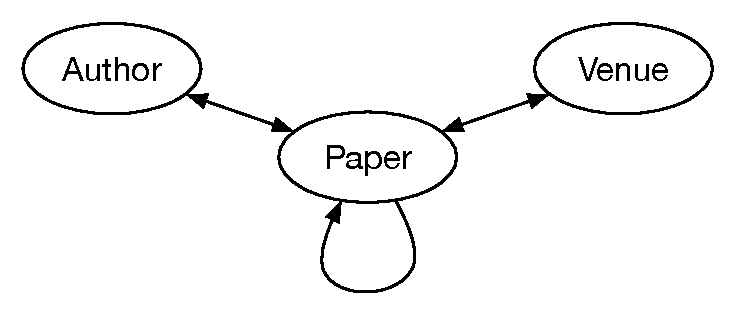
\includegraphics[trim = 0mm 0mm 0mm 0mm,width=0.45\hsize]{figs/publicationsSchema.pdf}
 \label{Fig:DBLP}
}
\subfigure[Movies Network]{
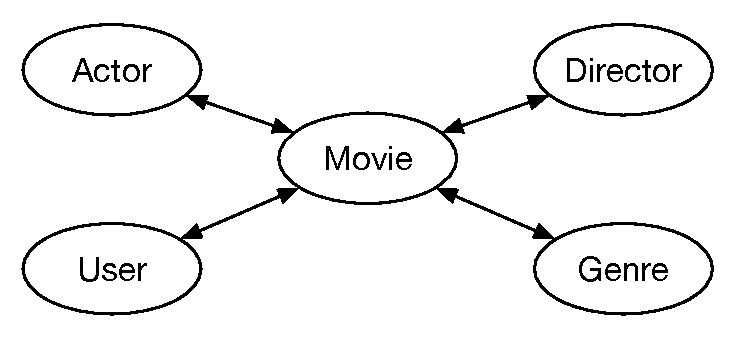
\includegraphics[trim = 0mm 0mm 0mm 0mm,width=0.45\hsize]{figs/moviesSchema.pdf}
 \label{Fig:IMDB}
}
\caption{The simplified network schema used for our experiments.} \label{Fig:expSchema}
\end{figure}


\begin{table}[t]
\centering
\caption{Publications dataset meta paths. $V$=\{Author, Paper, Venue\}.}
\label{table_publications}\scriptsize
\begin{tabular}{|c|l|} \hline
\textbf{Meta path} & \textbf{Meaning} \\ \hline

\textit{A--P--A} & [\textit{The target relation}] Authors are coauthors \\ \hline
\textit{A--P--V--P--A} & Authors publish in the same venue \\ \hline
\textit{A--P--A--P--A} & Authors have the same co-author \\ \hline
\textit{A--P--P--P--A} & Authors cite the same papers \\ \hline

\end{tabular}

\end{table}


\begin{table}[t]
\centering
\caption{Movies dataset meta paths. $V$=\{User, Movie, Actor, Director, Genre\}.}
\label{table_movies}\scriptsize
\begin{tabular}{|c|l|} \hline
\textbf{Meta path} & \textbf{Meaning} \\ \hline
\textit{U--M} & [\textit{The target relation}] A user watches a movie \\ \hline

\textit{U--M--A--M} & A user watches a movie with the same actor \\ \hline
\textit{U--M--D--M} & A user watches a movie with the same director \\ \hline
\textit{U--M--G--M} & A user watches a movie of the same genre \\ \hline
\textit{U--M--U--M} & A user watches a movie that another user  \\ \hline

\end{tabular}
\end{table}


\textit{Parameters.} $t$, $k$, ...

We consider $k$=3, 5, and 10 different time intervals for the dynamic analysis. In our evaluation, we execute the learned model on the last interval to measure the prediction accuracy.

\subsubsection{Evaluation Metrics.} 

To asses the link prediction accuracy, we use Area Under Curves (both Receiver Operating Characteristic (ROC) and Precision-Recall (PR) curves), termed as AUCROC and AUCPR \cite{davis2006relationship}. We also perform the non-parametric McNemar's test \cite{mcnemar1947note} to assess the statistical significance of the difference between the accuracy of different classifiers.

We performed 5-fold cross validation for the training phase.


\subsection{Results and Findings}

%DBLP
    179,607 authors had no co-author in 1996-2016. 
    78,635 authors had no co-author (about 4\%). 
    ------------
    100,972 (those who published in 1930-1996)?
    
    1,752,443 (total) - 100,972 = 1,651,471 (those who published in 1996-2016)?
    
    1,544,408 authors had no co-author in 1930-1996
    78,635 authors had no co-author (about 4\%). 
    ------------
    1,465,773 (those who published in 1996-2016)?

    1,752,443 (total) -1,465,773 = 300,000 (those who published in between)?
    
%    1,752,443 author_papervenuelist_map
%    2,811,533 paper_authorslist_map
%    10,163 venue_paperauthorslist_map
    
78,635 authors had no co-author (about 4\%)

Adding more features to our Logistic Regression model will increase the training accuracy because model has to consider more data to fit the logistic regression. But testing accuracy increases if feature is found to be significant

The null hypothesis of the McNemar's states that the same population proportion of links will be correctly classified by the two methods. However the test result gives a $p$-value $<$ 0.0001 and hence we reject the null hypothesis of equal classifier performance.

\amin{One reason that \textit{A--P--V--P--A} is better with intervals is that one may publish in ECIR but there are so many publishing there....}
